\section{Actividades y Metodología}

%Localización física y ubicación de instalaciones:

El proyecto se llevará a cabo en la Facultad de Ingeniería de la Universidad Nacional de La Plata.
Los ensayos necesarios se realizarán en el Área Técnica de Electrónica e Instrumental (ATEI)
del Departamento de Electrotecnia de la Facultad de Ingeniería de la UNLP.
Se realizarán consultas semanales con el tutor para el seguimiento del desarrollo del proyecto y
revisión de las decisiones tomadas por el equipo de trabajo.

Para alcanzar las metas y los objetivos propuestos, se realizarán las siguientes actividades:

\subsection{Estudio de bibliografía y diseño} \label{subsection:estudio_bibliografia}
Con el objetivo de capacitarse, se estudiarán y analizarán aspectos de seguridad, curvas de carga de la batería 
y topologías de conversores de potencia, de acuerdo con los requerimientos del proyecto. 
Se evaluarán las diferentes alternativas posibles y, en base a su complejidad y a su costo,
se elegirá la solución más adecuada para el logro de los objetivos. 

Se realizarán simulaciones en SPICE (programa de simulación con énfasis en circuitos integrados),
separando el proceso en 4 partes:
\begin{itemize}
    \item Fuente conmutada: Convierte la tensión alterna de la red doméstica en una tensión continua.
    \item Fuente de corriente: Brinda una corriente constante a la batería durante la primera etapa de carga.
    \item Circuito de control: Alterna entre las etapas de carga.
    \item Circuito de protección: Protege a la batería en caso de cortocircuito.
\end{itemize}

En la Figura \ref{fig:esquema_cargador} se puede observar un esquema en bloques del cargador.
El circuito de la fuente conmutada está compuesto por los bloques de rectificación, filtrado y conversión DC-DC.
El controlador se encarga de generar una señal PWM en base a la tensión y la corriente de la batería.
La referencia es una señal de corriente ya que la tensión nominal del cargador es fija.
El circuito de protección está integrado en el bloque de control.

Para disminuir las pérdidas de potencia en la etapa de corriente constante y obtener una mayor eficiencia, se modificó la estructura del cargador con respecto al diseño original. 
En primera instancia, para mantener la tensión a la salida del conversor en 42V, se propuso un ciclo de trabajo constante 
con el cual la caída de tensión en la etapa de control de corriente generaba una disipación de potencia excesiva.
Modificando el circuito de conversión que controla tanto la corriente como la tensión se evita una etapa posterior limitadora de corriente.

%incluir esquema de cargador
\begin{figure}
    \centering
    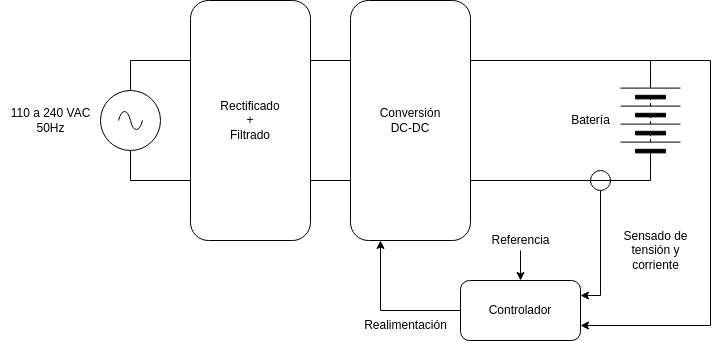
\includegraphics[width=\textwidth]{images/esquema_cargador_v2.png}
    \caption{Esquema del cargador}
    \label{fig:esquema_cargador}
\end{figure}

Se realizará un análisis crítico de las primeras simulaciones y, en base a los resultados obtenidos, 
se corregirán los circuitos propuestos. 
Esta etapa finaliza con la presentación del informe parcial. 

\subsection{Simulaciones}
El circuito fue diseñado y probado en LTSPICE (FALTA REFERENCIA), con el fin de verificar el diseño.
El proceso hasta el día de la fecha podría dividirse en las siguientes secciones:
\begin{enumerate}
    \item Simulación del conversor.
    \item Simulación del rectificador de entrada.
    \item Simulación del circuito de control.
    \item Simulación de distintos modelos de batería.
\end{enumerate}

En las siguientes secciones se detallarán cada una de estas etapas,
enumerando los problemas encontrados y las soluciones propuestas.

\subsubsection{Simulación del conversor}
El primer paso de diseño fue la elección de una topología de conversión DC-DC.
El conversor debe alcanzar una potencia máxima de 300W y debe ser lo más sencillo posible para evitar un costo elevado. 
La topología flyback es de baja complejidad al estar integrada por muy pocos componentes. 
Como desventajas, el tamaño del núcleo del transformador se incrementa con la potencia requerida y en bornes del
interruptor presenta una tensión igual al doble de la tensión máxima de entrada. En aplicaciones típicas se alcanzar valores de hasta 150W.
La topología forward con un solo switch disminuye el tamaño del núcleo del transformador. 
Como desventajas, al igual que el flyback presenta alta tensión en bornes del interruptor y se eleva el costo debido al agregado de la bobina de filtrado.
Admite una mayor potencia de salida entre 150-250W.
por lo que se optó por la topología forward con dos switches. 

Esta topología permite que la disipación de potencia por switch se reduzca a la mitad con respecto a
su contraparte de un solo switch y cuenta con un tamaño del transformador reducido con respecto a
un flyback de doble switch, ya que la energía no necesita almacenarse en el entrehierro.

El problema que presentó la utilización de un conversor de tipo forward con doble switch fue que
las señales que controlan a los switches son poco convencionales, lo cual se detallará en la secciones siguientes.

\subsubsection{Simulación del rectificador de entrada}
Una vez definido el circuito de conversión, se procedió a analizar los requisitos de la tensión de entrada.
Una primera aproximación fue la de utilizar un rectificador de onda completa con un filtro pasa bajos,
lo cual fue suficiente para esta aplicación.

En base a sugerencias de la cátedra, se analizó también la posibilidad de utilizar un rectificador controlado,
pero después de realizar las simulaciones correspondientes se llegó a la conclusión de que no daría ningún beneficio
significativo y acomplejaría demasiado el diseño del circuito.

% Agregar lo del criterio de selección del rectificador, creo que era lo de la potencia del capacitor
% pero no tengo idea como ponerlo

\subsubsection{Simulación del circuito de control}
Esta etapa fue la mas extensa en diseñar debido a su complejidad. Inicialmente solo debía realimentar la tensión de salida
y generar la señal PWM en base a esta, pero en base a los cambios descritos en la sección \ref{subsection:estudio_bibliografia}
se separó su diseño en tres etapas:

\begin{enumerate}
    \item Compensador y generador PWM
    \item Selector de modo de funcionamiento
    \item Controlador para los switches
\end{enumerate}

La primer etapa se implementó en base a las topologías descritas en \cite{mohan}. Se puede observar,
en la figura \ref{fig:esquema_compensador}, un modelo simplificado del circuito.

\begin{figure}
    \centering
    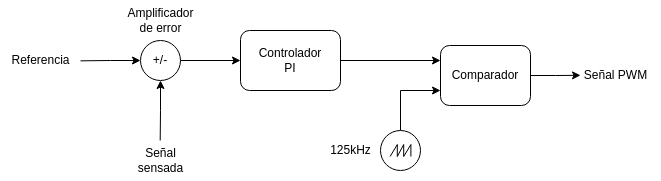
\includegraphics[width=\textwidth]{images/compensador.png}
    \caption{Esquema del compensador y el generador de señal PWM}
    \label{fig:esquema_compensador}
\end{figure}

Los parámetros del bloque proporcional-integrador (PI) fueron definidos a partir de valores típicos obtenidos de \cite{mohan}
y posteriormente ajustados para que el circuito funcione en las condiciones de la aplicación.
La frecuencia de switching es definida por la frecuencia de la señal de diente de sierra y también se tomó un valor típico.

\begin{figure}
    \centering
    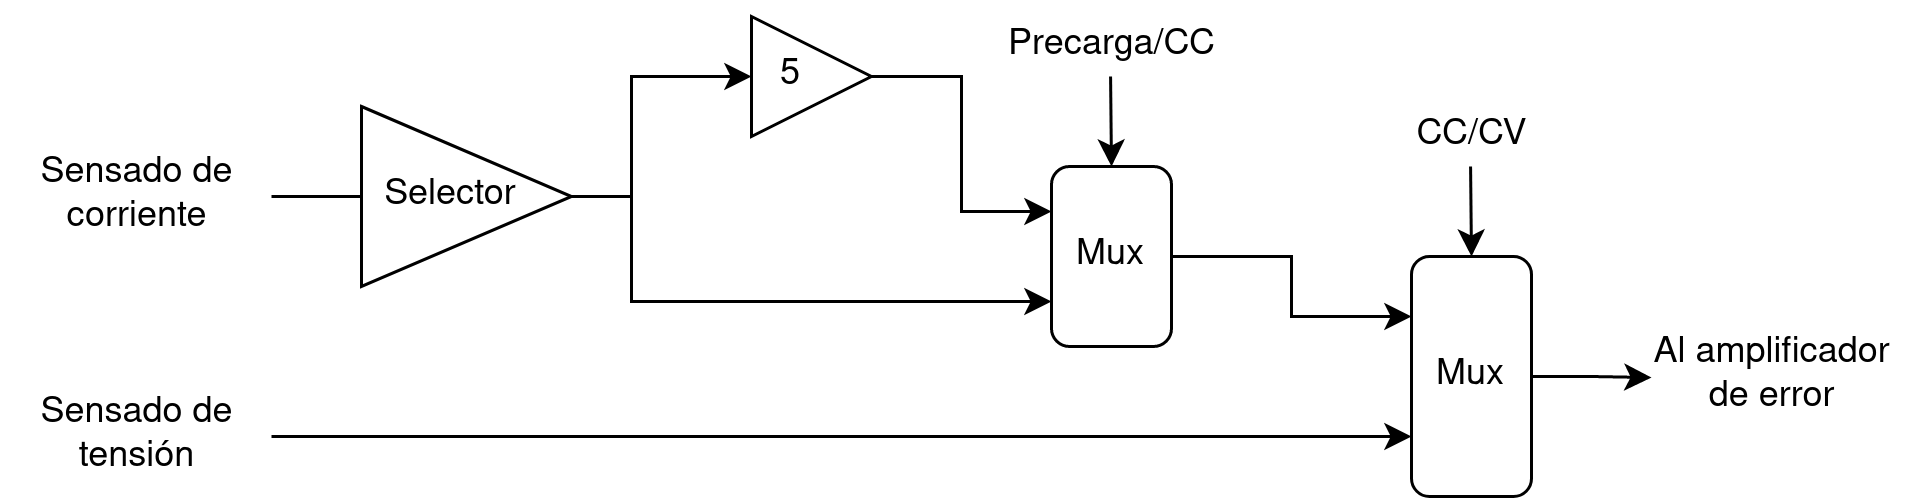
\includegraphics[width=\textwidth]{images/selector.png}
    \caption{Esquema del selector de modo}
    \label{fig:esquema_selector}
\end{figure}

Una vez diseñado el compensador, se procedió a diseñar el circuito de cambio de modo (Precarga, tensión constante y corriente constante).
En la figura \ref{fig:esquema_selector} se puede observar el esquema de este circuito.

Las señales de tensión y corriente están normalizadas con respecto a sus valores nominales.
Un amplificador de ganancia variable actúa como selector de corriente de salida,
modificando la amplitud de la señal de control de dicha variable.
La selección entre el modo de precarga y el modo de corriente constante se hace comparando el nivel de tensión de la batería
con una señal de referencia, siendo el segundo modo activado una vez que la tensión supera los 30V.
El bloque de ganancia 10 tiene como objetivo amplificar la señal de control, ya que la corriente de salida para el modo
de precarga es 10 veces mas chica que la de corriente constante.

La normalización de las señales nombrada anteriormente permite que la selección de la señal del último multiplexor
se haga en base a cual es la mayor de las dos. Esto, visto desde una perspectiva general, permite establecer un límite
tanto de tensión como de corriente de salida, lo cual es importante porque representa la base del método de carga.

Finalmente, para la selección de un controlador para los MOSFETs se tuvieron en cuenta algunos parámetros como
la tensión máxima de entrada, frecuencia de switching y sincronización de las señales,
pero no se logró hallar un controlador adecuado para esta aplicación.
El principal motivo fue que los controladores convencionales generan señales alternadas mediante el método de bootstrapping (REFERENCIA),
lo cual no sirve para la topología elegida. Esto, combinado con el elevado nivel de tensión en la entrada,
llevó a la búsqueda de otros métodos de control; por eso, se diseñó un controlador propio que se adaptara
a las necesidades del proyecto, cuyo diagrama puede observarse en la figura \ref{fig:driver}.

\begin{figure}
    \centering
    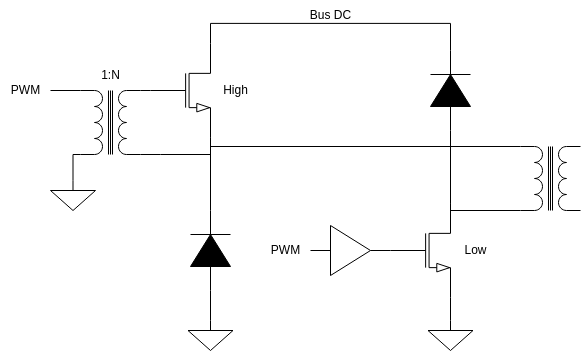
\includegraphics[width=\textwidth]{images/driver.png}
    \caption{Esquema del controlador de los MOSFETs}
    \label{fig:driver}
\end{figure}

\subsubsection{Simulación de distintos modelos de batería}
Para obtener resultados fiables de una simulación es necesario contar con un buen modelo.
Inicialmente se realizó un modelo de resistencia variable a partir de los datos confeccionados durante los ensayos,
el cual fue util para verificar el correcto funcionamiento de los límites de tensión y corriente,
pero a medida que el proyecto fue avanzando, dejó de ser representativo de la realidad y hubo que corregirlo.

El siguiente modelo propuesto fue un capacitor de muy alto valor, el cual permitiría agregar el parámetro de capacidad
de la batería. Este modelo no fue satisfactorio, por lo que se optó por la solución que actualmente se está utilizando:
Un modelo dinámico con resistencia interna, estado de carga y tensión de circuito abierto dependiente del estado de carga (REFERENCIA).


\subsection{Implementación}
Se diseñará un circuito impreso y se construirá un prototipo funcional que cumpla con las especificaciones propuestas. 
Debido a que el costo de una batería de litio de las características necesarias es elevado,
se evaluará la posibilidad de realizarlo a escala con una batería de menor tensión y/o capacidad.

\subsection{Validación}
Una vez terminado el proceso de diseño e implementación,
se verificará que el prototipo cumpla con las especificaciones presentadas.